\section{Kvantmekanik}

\paragraph{Brister i klassisk fysik}
Redan innan kvantmekaniken formulerades, fanns det brister i det experimentella beviset för den klassiska fysiken.

\subparagraph{Ultravioletta katastrofen}
Ett bevis var att den klassiska förutsägelsen av svartkroppsstrålning var
\begin{align*}
	I(\nu, T) = \frac{2kT\nu^{2}}{c^{2}},
\end{align*}
som divergerar för stora frekvenser. Observationer av svartkroppsstrålning var naturligtvis inte i närheten av detta utan gick mot $0$ även för höga frekvenser.

Max Planck sägs att ha upptäckt kvantmekaniken vid att härleda intensitetsfördelningen för svartkroppsstrålning under antagandet att energinivåerna i kroppen var diskreta kvanta av $h\nu$, där $h$ är den nu införda Plancks konstant. Han fick
\begin{align*}
	I(\nu, T) = \frac{2h\nu^{3}}{c^{2}}\frac{1}{e^{\frac{h\nu}{kT}} - 1}.
\end{align*}
Denna går både mot $0$ för höga frekvenser och beter sig som den klassiska förutsägelsen vid  låga frekvenser. Einstein gissade senare att $h\nu$ var energien för partiklarna som bygger upp ljus - fotoner.

\subparagraph{Fotoelektriska effekten}
Om man bestrålar metaller med elektromagnetisk strålning, frigörs elektroner (upptäckta vid det här laget) från metallet. Man kunne sätta metallet i närheten av en anod så att en spänningsskillnad mellan metallet och anoden kunde attrahera metaller till anoden. Vid at elektriskt koppla de två samman, kunde man mäta strömmen som orsakades av de frigjorda elektronerna. Det som observerades var:
\begin{itemize}
	\item Det frigjordes bara elektroner om den inkommande strålningen hade en frekvens över en viss gränsfrekvens.
	\item Under denna gränsfrekvensen spelade strålningsintensiteten ingen roll.
	\item Över gränsfrekvensen mättes den maximala elektronenergin som $E = h\nu - W$.
\end{itemize}

Detta var svårt att förklara med klassisk fysik.

\subparagraph{Comptonspridning}
Elektromagnetisk strålning kan spridas på elektroner. Klassiskt är det svårt att förklara spridningsmönstret som uppstår, eftersom elektromagnetisk strålning är vågor. Däremot kan man anta att strålningen består av fotoner med rörelsemängd och energi enligt speciell relativitetsteori och resultaten från fotoelektriska effekten, som illustrerad i figur \ref{fig:compton_collision}.

\begin{figure}[!ht]
	\centering
	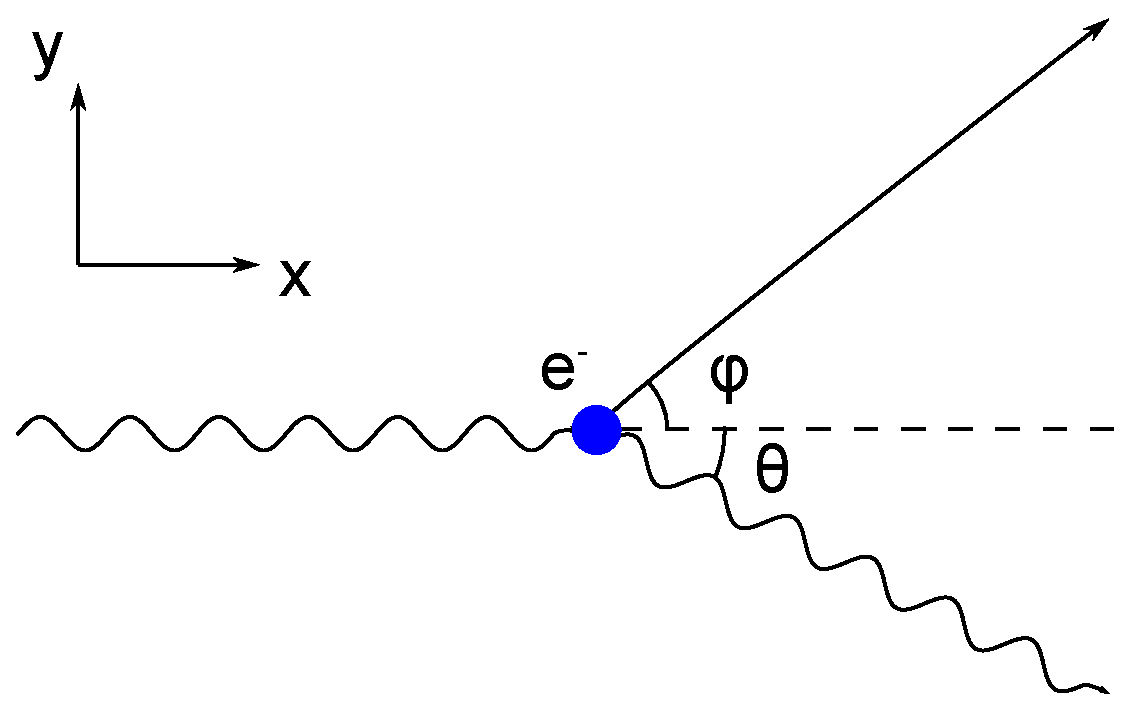
\includegraphics[width = 0.5\textwidth]{./Images/compton_collision.eps}
	\caption{Illustration av studs mellan en foton och en elektron.}
	\label{fig:compton_collision}
\end{figure}

Energins bevarande ger
\begin{align*}
	h\nu + m_{e, 0}c^{2} = E_{e} + h\nu'
\end{align*}
och rörelsemängdens bevarande ger
\begin{align*}
	h\frac{\nu}{c} = h\frac{\nu'}{c}\cos{\phi} + p_{e}'\cos{\theta}, \\
	h\frac{\nu'}{c}\sin{\phi} - p_{e}'\sin{\theta} = 0.
\end{align*}
Vi omformulerar förste rörelsemängdekvationen till
\begin{align*}
	h\frac{\nu}{c} - h\frac{\nu'}{c}\cos{\phi} = p_{e}'\cos{\theta}
\end{align*}
och kvadrerar för att få
\begin{align*}
	h^{2}\frac{\nu^{2}}{c^{2}} - 2h^{2}\frac{\nu\nu'}{c^{2}}\cos{\phi} + h^{2}\frac{\nu'^{2}}{c^{2}}\cos^{2}{\phi} = p_{e}'^{2}\cos^{2}{\theta}.
\end{align*}
Kombinerat med kvadratet av den andra rörelsemängdsekvationen ger detta
\begin{align*}
	h^{2}\frac{\nu^{2}}{c^{2}} + h^{2}\frac{\nu'^{2}}{c^{2}} - 2h^{2}\frac{\nu\nu'}{c^{2}}\cos{\phi} = p_{e}'^{2}.
\end{align*}
Energins bevarande ger vidare
\begin{align*}
	E_{e} = h\nu - h\nu' + m_{e, 0}c^{2}.
\end{align*}
Vi kvadrerar och kombinerar med massa-energi-sambandet från speciell relativitet och får
\begin{align*}
	h^{2}(\nu - \nu')^{2} + 2h(\nu - \nu')m_{e, 0}c^{2} + m_{e, 0}^{2}c^{4} &= p_{e}'^{2}c^{2} + m_{e, 0}^{2}c^{4} \\
	                                                                        &= h^{2}\nu^{2} + h^{2}\nu'^{2} - 2h^{2}\nu\nu'\cos{\phi} + m_{e, 0}^{2}c^{4}, \\
	(\nu - \nu')m_{e, 0}c^{2}                                               &= h\nu\nu'(1 - \cos{\phi}).
\end{align*}
Vi skriver nu om till våglängd och får
\begin{align*}
	(\frac{c}{\lambda} - \frac{c}{\lambda'})m_{e, 0}c^{2} &= h\frac{c^{2}}{\lambda\lambda'}(1 - \cos{\phi}), \\
	(\lambda' - \lambda)m_{e, 0}c                         &= h(1 - \cos{\phi}), \\
	\lambda' - \lambda                                    &= \frac{h}{m_{e, 0}c}(1 - \cos{\phi}),
\end{align*}
alternativt i termer av energi
\begin{align*}
	E' = \frac{1}{\frac{1 - \cos{\phi}}{m_{e, 0}c^{2}} + \frac{1}{E}},
\end{align*}
vilket stämde överens med experiment.

\paragraph{Röntgendiffraktion}
Röntgenstråler har ganska liten våglängd. För att få (klassisk) diffraktion med röntgenstråling, kan man använda plan av atomer i fasta material. Man kan visa att diffraktionsvillkoret är
\begin{align*}
	2d\sin{\theta} = n\lambda,
\end{align*}
där $\theta$ är infallsvinkeln för strålningen och $d$ är avståndet mellan atomplanen.

\paragraph{Röntgenspektra}
Om ett metall bestrålas av röntgenstrålning med olika våglängder, kan man använda en diffraktionsuppställning och mäta intensiteten som funktion av utgående vinkel. Eftersom man har ett spektrum av våglängder, får man konstruktiv interferens i ett intervall av vinklar. Braggs formel implicerar att den utgående vinkeln beror av våglängden till strålningen som interfererar konstruktivt, varför man (typ) kan plotta ett spektrum från ett sådant experiment som i figur \ref{fig:x-ray_spectrum}.

\begin{figure}[!ht]
	\centering
	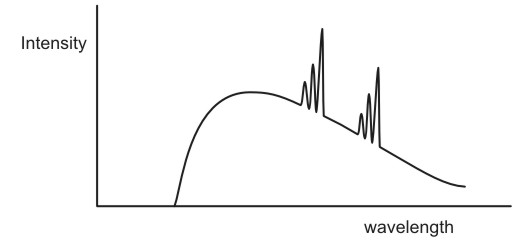
\includegraphics[width = 0.5\textwidth]{./Images/x-ray_spectrum.jpg}
	\caption{Typiskt röntgenspektrum.}
	\label{fig:x-ray_spectrum}
\end{figure}

Röntgenspektrumet är en superposition av ett kontinuerligt spektrum och vissa skarpa toppar. Den kontinuerliga delen kommer direkt från våglängdsspektrumet. De skarpa topparna 
kommer från exitationer av elektroner i metallet. När metallernas elektroner exiteras, skapas det en foton när de hoppar tillbaka till tillståndet med lägre energi, och detta orsakar intensitetstopparna.

\paragraph{de Broglie-våglängd}
Kombinationen
\begin{align*}
	E = h\nu, p = \frac{E}{c}
\end{align*}
för fotoner fick de Broglie att hypotetisera att alla partiklar har en våglängd. Vid att kombinera resultaten ovan, var de Broglies hypotes att denna våglängden ges av
\begin{align*}
	\lambda = \frac{h}{p}.
\end{align*}
Detta kan i stället omformuleras till kinetisk energi vid att använda att
\begin{align*}
	p^{2} &= \frac{1}{c^{2}}E^{2} - m_{0}^{2}c^{2} \\
	      &= \frac{1}{c^{2}}(T^{2} + m_{0}^{2}c^{4} + 2Tm_{0}c^{2}) - m_{0}^{2}c^{2} \\
	      &= \frac{T^{2}}{c^{2}} + 2Tm_{0}, \\
	p     &= \sqrt{2Tm_{0} + \left(\frac{T}{c}\right)^{2}},
\end{align*}
vilket ger
\begin{align*}
	\lambda &= \frac{h}{\sqrt{2Tm_{0} + \left(\frac{T}{c}\right)^{2}}} \\
	        &= \frac{h}{\sqrt{2Tm_{0}}}\frac{1}{\sqrt{1 + \left(\frac{T}{c\sqrt{2Tm_{0}}}\right)^{2}}} \\
	        &= \frac{h}{\sqrt{2Tm_{0}}}\frac{1}{\sqrt{1 + \left(\frac{\sqrt{T}}{c\sqrt{2m_{0}}}\right)^{2}}} \\
	        &= \frac{h}{\sqrt{2Tm_{0}}}\frac{1}{\sqrt{1 + \frac{T}{2m_{0}c^{2}}}}.
\end{align*}

\paragraph{Davidsson-Germers experiment}
I detta experimentet bestrålades en nickelkatod normalt på sin yta med elektroner som accelererades med någon spänning, och reflekterade elektroner detekterades som funktion av vinkel ut från strålen. I detta experimentet uppmättes ett intensitetsmaximum vid en annan vinkel än $0$, och med Braggs formel samsvarar detta maximumet med avståndet mellan atomplan i nickel.

\paragraph{Osäkerhetsprincipen}
de Broglies hypotes säjer att $p$ beror av partikelvågors våglängd i $x$ och $E$ av partikelvågors våglängd i $t$. Vad är en våglängd i $t$? Jo, avståndet i tid mellan två lika punkter på vågen, vilket är perioden, som är direkt kopplad till frekvensen. Detta kombinerad med satser från Fourieranalys implicerar
\begin{align*}
	\Delta p \Delta x \geq \frac{\hbar}{2}, \\
	\Delta E \Delta t \geq \frac{\hbar}{2},
\end{align*}
där vi har infört den reducerade Plancks konstant $\hbar = \frac{h}{2\pi}$.

\paragraph{Vågfunktionen}
Baserad på dessa resultat infördes vågfunktionen $\Psi$. Det postulerades vidare att för alla dynamiska system existerar en vågfunktion som innehåller all information om systemet.
Denna är kontinuerligt deriverbar.

\paragraph{Sannolikhet}
Olika experiment började visa att partiklars position har ett icke-deterministiskt element i sig. Positionen beskrivs av en täthetsfunktion, som postulerades vara $\abs{\Psi}^{2}$.

\paragraph{Schrödingerekvationen}
För ett system av en partikel i en dimension som rör sig i en potential $V$ beskrivs vågfunktionen av
\begin{align*}
	-\frac{\hbar^{2}}{2m}\del{x}{\del{x}{\Psi}} + V\Psi = i\hbar\del{t}{\Psi}.
\end{align*}
Detta kan utvidgas för mer allmäna system till
\begin{align*}
	\hat{H}\Psi = i\hbar\del{t}{\Psi},
\end{align*}
där $\hat{H}$ är systemets Hamiltonoperator, som kommer diskuteras sedan.

\paragraph{Stationära tillstånd}
Gör ansatsen $\Psi = \psi(x)\phi(t)$. Då ger Schrödingerekvationen för en enda partikel
\begin{align*}
	-\frac{\hbar^{2}}{2m}\phi\del{x}{\del{x}{\psi}} + V\psi\phi = i\hbar\psi\del{t}{\phi}.
\end{align*}
Detta kan separeras till
\begin{align*}
	-\frac{\hbar^{2}}{2m}\frac{\del{x}{\del{x}{\psi}}}{\psi} + V = i\hbar\frac{\del{t}{\phi}}{\phi}.
\end{align*}
Om potentialen är tidsoberoende, är vänstersidan bara en funktion av position och högersidan bara en funktion av tid. Därmed måste båda sidor vara lika med en konstant, som vi för tillfället kallar $E$.

Tidsberoendet ger
\begin{align*}
	\del{t}{\phi} &= -i\frac{E}{\hbar}\phi, \\
	\phi          &= Ae^{-i\frac{E}{\hbar}t}.
\end{align*}
Om vi tittar på frekvensen, får vi
\begin{align*}
	\nu = \frac{1}{2\pi}\frac{E}{\hbar} = \frac{E}{h},
\end{align*}
och vi ser att $E$ precis motsvarar partikelvågens energi. Vi noterar vidare att $\abs{\phi}^{2}$ är tidsoberoende, så denna sortens tillstånd ändrar sig inte med tiden.

Positionsberoendet ger nu
\begin{align*}
	-\frac{\hbar^{2}}{2m}\del{x}{\del{x}{\psi}} + V\psi = E\psi.
\end{align*}
Alla lösningarna till denna ekvationen är egenfunktioner till operatorn $-\frac{\hbar^{2}}{2m}\del{x}{} + V$ med egenvärde $E$. Utöver detta kan inget säjas utan information om potentialen.

\paragraph{Väntevärde och operatorer}
Eftersom kvantmekaniken handlar om sannolikheter, är även konceptet väntevärde relevant. I kvantmekaniken postulerar vi att det till varje observabel $q$ finns en operator $\hat{q}$, och dens väntevärde ges av
\begin{align*}
	\expval{q} = \integ{}{x}{\cc{\psi}\hat{q}\psi}.
\end{align*}
Exempel på grundläggande operatorer är
\begin{itemize}
	\item positionsoperatorn $\hat{x} = x$.
	\item rörelsemängdsoperatorn $\hat{p}_{i} = -i\hbar\del{i}{}$.
	\item kinetisk energi-operatorn $\hat{T} = \frac{1}{2m}\hat{p}^{2}$.
	\item potentialoperatorn $\hat{V} = V$.
	\item Hamiltonoperatorn $\hat{H} = \hat{T} + \hat{V}$.
	\item rörelsemängdsmomentoperatorn $\hat{L}_{i} = \leci{ijk}\hat{r}_{j}\hat{p}_{k}\Leftrightarrow \hat{\vb{L}} = \hat{\vb{r}}\times\hat{\vb{p}}$.
\end{itemize}

\paragraph{Spinn}
Spinn är en ny fysikalisk storhet som dyker upp i kvantmekaniska sammanhang. Den har egenvärden
\begin{align*}
	\abs{S} = \sqrt{s(s + 1)}\hbar
\end{align*}
enligt postulat, där $s$ är ett nytt kvanttal. För elektroner är $s = \frac{1}{2}$.

Alternativt kan man titta på $z$-komponenten av spinnet, med egenvärden
\begin{align*}
	S_{z} = m_{s}\hbar,
\end{align*}
där $m_{s} = 0, \dots, \pm s$ är det spinnmagnetiska kvanttalet.

\paragraph{Fermioner och bosoner}
Alla partiklar kan delas upp i bosoner och fermioner. Om man betraktar den simultana vågfunktionen $\Psi_{1, 2}$ till två lika partiklar, är dessa bosoner om $\Psi_{1, 2} = \Psi_{2, 1}$ och fermioner om $\Psi_{1, 2} = -\Psi_{2, 1}$.

\paragraph{Pauliprincipen}
Fermionerna uppfyller Pauliprincipen, som säger att två ej särskiljbara partiklar ej kan existera i samma individuella kvanttillstånd. Ett typiskt exempel på en fermion är en elektron.

En konsekvens av detta är det faktum att grundämnerna delas upp i periodiska systemet på det sättet de gör.

\paragraph{Magnetiskt moment}
Det magnetiska momentet som skapas av en strömslinga ges av
\begin{align*}
	\vb{\bm{\mu}} = IA\vb{e}_{\text{n}},
\end{align*}
där $I$ är strömmen i slingan, $A$ är ytan som slingan omkransar och $\vb{e}_{\text{n}}$ är en enhetsvektor normalt på slingan enligt högerhandsregeln.

\paragraph{Spinn-bankoppling}
Betrakta en elektron i en cirkulär bana kring en proton. I elektronens system rör protonen sig åt motsatt håll, och dens rörelse orsakar en ström
\begin{align*}
	I &= \frac{e}{T} \\
	  &= \frac{e}{\frac{2\pi r}{v}} \\
	  &= \frac{em_{e}vr}{2\pi m_{e}r^{2}} \\
	  &= \frac{e}{2\pi m_{e}r^{2}}L,
\end{align*}
där $L$ är belopppet av elektronens rörelsemängdsmoment. Det orsakade magnetfältet har flödestäthet
\begin{align*}
	\vb{B} &= -\frac{\mu_{0} I}{2r}\vb{e}_{\text{n}} \\
	       &= -\frac{\mu_{0}}{2r}\frac{e}{2\pi m_{e}r^{2}}\vb{L} \\
	       &= -\frac{\mu_{0}e}{4\pi m_{e}r^{2}}\vb{L}.
\end{align*}
Detta orsakar en potential
\begin{align*}
	V = \vb{\bm{\mu}}_{s}\cdot\vb{B} = -\frac{\mu_{0}e^{2}}{4\pi m_{e}^{2}r^{3}}\vb{S}\cdot\vb{L}.
\end{align*}
Vi ser alltså att den orsakade potentialen beror av elektronens spinn och dens rörelsemängdsmoment. Detta är spinn-bankoppling.

\paragraph{Oändlig lådpotential}
För att få en känsla för vilken sorts fysik som kommer ut av kvantmekaniken, betraktar vi en partikel i en oändlig lådpotential, dvs.
\begin{align*}
	V = 
	\begin{cases}
		0,      &0 < x < a, \\
		\infty, &\text{annars.}
	\end{cases}
\end{align*}
Detta motsvarar en låda med oändligt starka väggar. Rumdelen av Schrödingerekvationen för stationära tillstånd ger inuti lådan
\begin{align*}
	-\frac{\hbar^{2}}{2m}\del{x}{\del{x}{\psi}} &= E\psi, \\
	\del{x}{\del{x}{\psi}}                      &= -\frac{2mE}{\hbar^{2}}\psi.
\end{align*}
Vi definierar nu
\begin{align*}
	k^{2} = \frac{2mE}{\hbar^{2}}
\end{align*}
och får
\begin{align*}
	\del{x}{\del{x}{\psi}} = -k^{2}\psi.
\end{align*}
Detta har lösningar
\begin{align*}
	\psi = Ae^{ikx} + Be^{-ikx}.
\end{align*}

För att få mer information, behövs randvillkor. På grund av vågfunktionens krökningsegenskaper, som framkommer av Schrödingerekvationen, måste vi ha $\psi(0) = \psi(a) = 0$. Första randvillkoret ger
\begin{align*}
	A + B &= 0, \\
	\psi  &= A\sin{kx}.
\end{align*}
Andra randvillkoret ger
\begin{align*}
	ka = n\pi.
\end{align*}
Nu kan energin bestämmas enligt
\begin{align*}
	\frac{n^{2}\pi^{2}}{a^{2}} &= \frac{2mE}{\hbar^{2}}, \\
	E                          &= \frac{\hbar^{2}n^{2}\pi^{2}}{2ma^{2}},
\end{align*}
och vi ser att energin kan bara anta vissa diskreta värden. Vi ser även att grunntilståndets energi är nollskild, som indikerar att ett system som beskrivs av kvantmekaniken alltid kommer ha en viss rörelse.

Slutligen ger normaliseringsvillkoret
\begin{align*}
	\inteval{0}{a}{x}{\abs{B}^{2}\sin^{2}{kx}} = 1.
\end{align*}
Integralen på vänstersidan är
\begin{align*}
	\abs{B}^{2}\inteval{0}{a}{x}{\frac{1 - \cos{2kx}}{2}}.
\end{align*}
Den andra termen ger inget bidrag eftersom den har period $a$, och detta ger
\begin{align*}
	\abs{B}^{2}\frac{a}{2} &= 1, \\
	\abs{B}                &= \sqrt{\frac{2}{a}}.
\end{align*}
Observera att vi endast skriver absolutbeloppet eftersom $B$ kan innehålla en komplex fas utan att det ändrar fysiken.

\paragraph{Ändlig lådpotential}
Betrakta en partikel i en ändlig lådpotential, dvs.
\begin{align*}
	V = 
	\begin{cases}
		0,      &0 < x < a, \\
		V_{0},  &\text{annars.}
	\end{cases}
\end{align*}
Detta motsvarar en låda med en viss ``flexibilitet'' i väggarna. Rumdelen av Schrödingerekvationen för stationära tillstånd ger inuti lådan
\begin{align*}
	\del{x}{\del{x}{\psi}} = -\frac{2mE}{\hbar^{2}}\psi.
\end{align*}
och utanför lådan
\begin{align*}
	\del{x}{\del{x}{\psi}} = -\frac{2m(V_{0} - E)}{\hbar^{2}}\psi.
\end{align*}
Vi definierar som förut
\begin{align*}
	k^{2} = \frac{2mE}{\hbar^{2}},\ \alpha^{2} = \frac{2m(V_{0} - E)}{\hbar^{2}}.
\end{align*}
Om $E < V_{0}$ är lösningarna
\begin{align*}
	\psi =
	\begin{cases}
		Ae^{\alpha x} + A'e^{-\alpha x}, &x < 0, \\
		B\sin{kx} + C\cos{kx},           &0 < x < a, \\
		De^{-\alpha x} + D'e^{\alpha x}, &a < x.
	\end{cases}
\end{align*}
Vi sätter direkt $A' = D' = 0$ eftersom dessa termerna skulle ge lösningar som inte är normaliserbara.

Vi ser från lösningen att en partikel kan penetrera lite in i en region där dens totala energi är negativ, det så kallade klassiskt förbjudna området. Vi kan även definiera ett penetrationsdjup
\begin{align*}
	\delta = \frac{1}{\alpha} = \frac{\hbar}{\sqrt{2m(E - V_{0})}}
\end{align*}
som ett mått på hur långt in i den klassiskt förbjudna sonen bundna tillstånd kan penetrera.

Vi är vidare intresserade av villkoret för energin. För att få detta, använder vi att $\psi$ är kontinuerligt deriverbar, vilket ger:
\begin{align*}
	&A = C, \\
	&B\sin{ka} + C\cos{ka} = De^{-\alpha a}, \\
	&A\alpha = kB, \\
	&k(B\cos{ka} - C\sin{ka}) = -\alpha De^{-\alpha a}.
\end{align*}
Insättning av första och tredje ekvationen i andra och fjärde ger
\begin{align*}
	\frac{\alpha}{k}A\sin{ka} + A\cos{ka} = De^{-\alpha a}, \\
	\alpha A\cos{ka} - kA\sin{ka} = -\alpha De^{-\alpha a}.
\end{align*}
Kvoten av dessa är
\begin{align*}
	\frac{\alpha\cos{ka} - k\sin{ka}}{\frac{\alpha}{k}\sin{ka} + \cos{ka}} = -\alpha.
\end{align*}
Vi definierar $x = \frac{k}{\alpha}$ och får
\begin{align*}
	\frac{\cos{ka} - x\sin{ka}}{\frac{1}{x}\sin{ka} + \cos{ka}} &= -1, \\
	\frac{\cot{ka} - x}{\frac{1}{x} + \cot{ka}}                 &= -1, \\
	\cot{ka} - x                                                &= -\frac{1}{x} - \cot{ka}, \\
	2\cot{ka}                                                   &= \frac{k}{\alpha} - \frac{\alpha}{k}.
\end{align*}
Detta är ett lite komplicerad kvantiseringsvillkor, men ändå ett sådant.

\paragraph{Andra potentialer}
Det finns andra intressanta potential att betrakta som kan användas för att beskriva fysikaliska system. Exempel är
\begin{itemize}
	\item det harmoniska potentialet $V = \frac{1}{2}Kx^{2}$, med energiegenvärden $E_{n} = \left(n + \frac{1}{2}\right)\hbar\omega_{0}$, där $\omega_{0} = \sqrt{\frac{K}{m}}$.
\end{itemize}

\paragraph{Bundna system}
Ett bundet system är ett system som är lokaliserad i rummet.

\paragraph{Obundna system}
Ett obundet system är ett system som ej är lokaliserad i rummet.

\paragraph{Ändlig barriär}
Betrakta en partikel i en ändlig lådpotential, dvs.
\begin{align*}
	V = 
	\begin{cases}
		V_{0}, &0 < x < a, \\
		0,     &\text{annars.}
	\end{cases}
\end{align*}
Man kan definiera en transmissionskoefficient och en reflektionskoefficient lika med sannolikheten för att partiklar transmitteras och reflekteras av barriären. För $E > V_{0}$ ges dessa av
\begin{align*}
	R &= \frac{\sin[2](\frac{\sqrt{2m(E - V_{0})}a}{\hbar})}{\sin[2](\frac{\sqrt{2m(E - V_{0})}a}{\hbar}) + 4\frac{E}{V_{0}}\left(\frac{E}{V_{0}} - 1\right)}, \\
	T &= \frac{4\frac{E}{V_{0}}\left(\frac{E}{V_{0}} - 1\right)}{\sin[2](\frac{\sqrt{2m(E - V_{0})}a}{\hbar}) + 4\frac{E}{V_{0}}\left(\frac{E}{V_{0}} - 1\right)}.
\end{align*}
För $E < V_{0}$ ges de av
\begin{align*}
	R &= \frac{\sinh[2](\frac{\sqrt{2m(E - V_{0})}a}{\hbar})}{\sinh[2](\frac{\sqrt{2m(E - V_{0})}a}{\hbar}) + 4\frac{E}{V_{0}}\left(1 - \frac{E}{V_{0}}\right)}, \\
	T &= \frac{4\frac{E}{V_{0}}\left(1 - \frac{E}{V_{0}}\right)}{\sinh[2](\frac{\sqrt{2m(E - V_{0})}a}{\hbar}) + 4\frac{E}{V_{0}}\left(1 - \frac{E}{V_{0}}\right)}.
\end{align*}

\paragraph{Tunneling}
Klassiskt kan en partikel inte kryssa en barriär om den har för låg energi. Kvantmekaniskt kan man beräkna en transmissionssannolikhet för tunneling.

Ett enkelt fall som illustrerar tunneling är potential som är konstant lika med $0$ förutom i en region med brädd $a$, där potentialen är $V_{0}$. Schrödingerekvationen ger för detta fallet
\begin{align*}
	T \approx 16\frac{E}{V_{0}}\left(1 - \frac{E}{V_{0}}\right)e^{-\frac{2a\sqrt{2m(V_{0} - E)}}{\hbar}}, E < V_{0}, a >> \delta,
\end{align*}
där $\delta$ är penetrationsdjupet som definierades i delen om ändlig lådpotential.

Tunneling som fenomen förklarar t.ex. $\alpha$-sönderfall, mikroskopitekniken STM och varför Solen brinner (fusion möjliggörs av att olika atomer kan tunnelera in i varandras kärnor).

\paragraph{Schrödingerekvationen i högre dimensioner}
I högre dimensioner utvidgas Schrödingerekvationen triviellt genom att utvidga definitionen av Hamiltonoperatorn till att verka i alla dimensioner. Även normaliseringen görs över alla dimensioner. Notera att separeringen i tid och rum är exakt likadan.

Ett enkelt exempel är för en partikel, där Hamiltonoperatorn utvidgas till
\begin{align*}
	\hat{H} = -\frac{\hbar^{2}}{2m}\laplacian + V.
\end{align*}